% !Mode:: "TeX:UTF-8"
\documentclass[newtxmath=true,newgeometry=two,capcenterlast=true,subcapcenterlast=true,openright=true,absupper=true,fontset=windowsnew,type=master]{hithesis}
% 此处选项中不要有空格
%%%%%%%%%%%%%%%%%%%%%%%%%%%%%%%%%%%%%%%%%%%%%%%%%%%%%%%%%%%%%%%%%%%%%%%%%%%%%%%%
% 必填选项
% type=doctor|master|bachelor
%%%%%%%%%%%%%%%%%%%%%%%%%%%%%%%%%%%%%%%%%%%%%%%%%%%%%%%%%%%%%%%%%%%%%%%%%%%%%%%%
% 选填选项(选填选项的缺省值已经尽可能满足了大多数需求,除非明确知道自己有什么
% 需求)
% glue=true|false
% 	含义:由于我工规范中要求字体行距在一个闭区间内,这个选项为true表示tex自
% 	动选择,为false表示区间内一个最接近版心要求行数的要求的默认值,缺省值为
% 	false。
% tocfour=true|false
% 	含义:是否添加第四级目录,只对本科文科个别要求四级目录有效,缺省值为
% 	false
% fontset=siyuan|windowsnew|windowsold
% 	含义:注意这个选项视为了解决特殊问题而设置,比如用有些发行版本的linux排
% 	版时可能(大多数发行版不会)会遇到的字体无法载入的问题,或者字体载入之
% 	后出现无法复制的问题以及想要解决排版如 biang biang 面的 biang 这类中易
% 	宋体无法识别的汉字的问题。没有特殊的需要不推荐使用这个选项。
%
% 	如果是安装了 windowns 字体的 linux 系统,可以填写windowsnew(win vista
% 	以后 的字体)或 windowsold(vista 以前)或者想用思源宋体并且是已经安装
% 	了思源宋体的任何系统,填写siyuan选项。缺省值为空,自动识别系统并匹配字体
% 	。模板版中给出的思源字体定义文件定义的思源字体的版本是Adobe版,其他字体
% 	是windowsnew字体。
% tocblank=true|false
% 	含义:目录中第一章之前,是否加一行空白。缺省值为true。
% chapterhang=true|false
% 	含义:目录的章标题是否悬挂居中,规范中要求章标题少于15字,所以这个选项
% 	有无没什么用,除了特殊需求。缺省值为true。
% fulltime=true|false
% 	含义:是否全日制,缺省值为true。非全日制如同等学力等,要在cover中设置类
% 	型,封面中不同格式
% subtitle=true|false
% 	含义:论文题目是否含有副标题,缺省值为false,如果有要在cover中设置副标
% 	题内容,封面中显示。
% newgeometry=one|two
% 	含义:规范中的自相矛盾之处,版芯是否包含页眉页脚,旧方法是按照包含页眉
% 	页脚来设置。该选项是多选选项,如果没有这个选项,缺省值是旧模板的版芯设
% 	置方法,如果设置该选项one或two,分别对应两种页眉页码对应版芯线的相对位
% 	置。第一种是严格按照规范要求,难看。第二种微调了页眉页码位置,好一点。
% debug=true|false
% 	含义:是否显示版芯框和行号,用来调试。默认否。
% openright=true|false
% 	含义:博士论文是否要求章节首页必须在奇数页,此选项不在规范要求中,按个
% 	人喜好自行决定。 默认否。注意,窝工的默认情况是打印版博士论文要求右翻页
% 	,电子版要求非右翻页且无空白页。如果想DIY(或身不由己DIY)在什么地方右
% 	翻页,将这个选项设置为false,然后在目标位置添加`\cleardoublepage`命令即
% 	可。
% capcenterlast=true|false
% 	含义:图题、表题最后一行是否居中对齐(我工规范要求居中,但不要求居中对
% 	齐),此选项不在规范要求中,按个人喜好自行决定。默认否。
% subcapcenterlast=true|false
% 	含义:子图图题最后一行是否居中对齐(我工规范要求居中,但不要求居中对齐
% 	),此选项不在规范要求中,按个人喜好自行决定。默认否。
% absupper=true|false
%       含义:中文目录中的英文索引在中文目录中的大小写样式歧义,在规范中要求首
%       字母大写,在work样例中是全大写。该选项控制是否全大写。默认否。
% bsmainpagenumberline=true|false
%       含义:由于本科生论文官方模板的页码和页眉格式混乱,提供这个选项自定义设
%       置是否在正文中显示页码横线,默认否。
% bsfrontpagenumberline=true|false
%       含义:由于本科生论文官方模板的页码和页眉格式混乱,提供这个选项自定义设
%       置是否在前文中显示页码横线,默认否。
% bsheadrule=true|false
%       含义:由于本科生论文官方模板的页码和页眉格式混乱,提供这个选项自定义设
%       置是否显示页眉横线,默认显示。
% splitbibitem=true|false
%       含义:参考文献每一个条目内能不能断页,应广大刀客要求添加。默认否。
% newtxmath=true|false
%       含义:数学字体是否使用新罗马。默认是。
%%%%%%%%%%%%%%%%%%%%%%%%%%%%%%%%%%%%%%%%%%%%%%%%%%%%%%%%%%%%%%%%%%%%%%%%%%%%%%%%

\usepackage{hithesis}
\graphicspath{{figures/}}

\begin{document}

\frontmatter
% !Mode:: "TeX:UTF-8"

\hitsetup{
  %******************************
  % 注意:
  %   1. 配置里面不要出现空行
  %   2. 不需要的配置信息可以删除
  %******************************
  %
  %=====
  % 秘级
  %=====
  statesecrets={公开},
  natclassifiedindex={TM301.2},
  intclassifiedindex={62-5},
  %
  %=========
  % 中文信息
  %=========
  ctitleone={局部多孔质气体静压},%本科生封面使用
  ctitletwo={轴承关键技术的研究},%本科生封面使用
  ctitlecover={面向自动驾驶系统测试用例生成的对抗生成网络和图像风格转换技术的实证研究},%放在封面中使用,自由断行
  ctitle={面向自动驾驶系统测试用例生成的对抗生成网络和图像风格转换技术的实证研究},%放在原创性声明中使用
  csubtitle={一条副标题}, %一般情况没有,可以注释掉
  cxueke={工学},
  csubject={计算机技术},
  caffil={创新创业学院},
  cauthor={闫施违},
  csupervisor={张煜群},
  % 日期自动使用当前时间,若需指定按如下方式修改:
  %cdate={超新星纪元},
  cstudentid={11749199},
  cstudenttype={同等学力人员}, %非全日制教育申请学位者
  %(同等学力人员)、(工程硕士)、(工商管理硕士)、
  %(高级管理人员工商管理硕士)、(公共管理硕士)、(中职教师)、(高校教师)等
  %
  %
  %=========
  % 英文信息
  %=========
  etitle={An empirical study of GANs and Neural Style Transfers for test case generation in autonomous driving system},
  esubtitle={This is the sub title},
  exueke={Engineering},
  esubject={Computer Technology},
  eaffil={\emultiline[t]{School of Innovation and Entrepreneurship}},
  eauthor={Shiwei Yan},
  esupervisor={Professor Yuqun Zhang},
  % 日期自动生成,若需指定按如下方式修改:
  edate={December, 2017},
  estudenttype={Master of Art},
  %
  % 关键词用“英文逗号”分割
  ckeywords={自动驾驶, 深度学习, 对抗生成网络, 图像风格转换},
  ekeywords={autonomous driving, deep learning, GAN, neural style transer},
}

\begin{cabstract}

近年来,得益于深度学习的发展,自动驾驶的研究与开发也取得了巨大的突破。国内外的许多公司都开发了自己的自动驾驶系统框架,譬如Google公司的Waymo,Baidu公司的Apollo和Tesla公司研制的Autopilot,其中最为人熟知的Autopilot已经成功的部署运行在了现实商用的Tesla轿车中。

尽管各大公司都标榜如今的自动驾驶系统安全性能已经足够高,但是近一两年发生的几起自动驾驶车祸引起了人们对于自动驾驶系统安全性能的关注,下左图是于2018年3月23号,发生在美国加州山景城高速公路上的一起车祸,事后事故分析指出由于Autopilot未能识别灰色公路背景下的白色防护栏从而导致的车祸的发生。同样的右图也是由于Uber公司研制的自动驾驶系统的误判,于2017年发生在美国亚利桑那州天普城的一起车祸。

\begin{figure}[h]
  \centering
  \subfigure[车祸1]{
          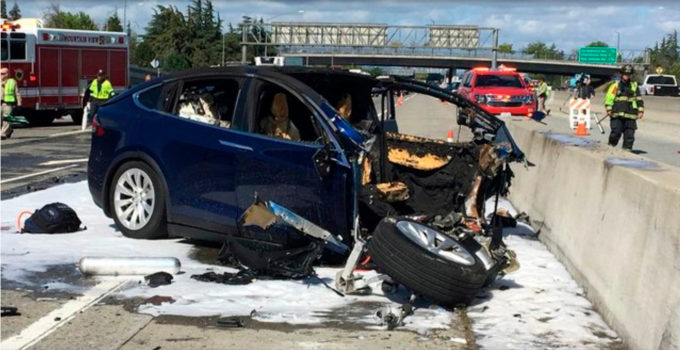
\includegraphics[width=0.45\textwidth, height=4cm]{crash_t}
  }
  \subfigure[车祸2]{
          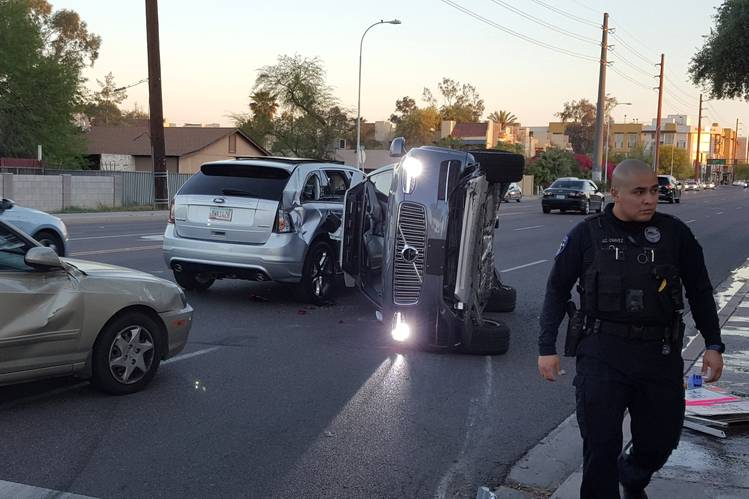
\includegraphics[width=0.45\textwidth, height=4cm]{crash_u}
  }
  \caption{crashs}
\end{figure}

除了上述之外,近年来还陆续有自动驾驶相关的车祸发生,以上种种都表明当前的自动驾驶的安全性能并没有人们认为的那么高。为了提升自动驾驶系统的安全等级,工业界和学术界都在此做了很多研究,于2017年学术界在此领域先后发表了2篇重要的文章,DeepXplore\cite{DeepXplore}和DeepTest\cite{DeepTest},DeepXplore提出了一套深度学习系统测试用例自动生成的框架。DeepTest延伸了DeepXplore的工作并将前者的方法成功的运用到了自动驾驶系统测试用例,即驾驶路况场景图,生成中,两者的工作都以现实的自动驾驶框架为测试对象,成功生成除了很多自动驾驶系统会误判的测试用例,这对提升自动驾驶系统的安全性能有着重大意义。

基于DeepXplore和DeepTest的工作,我所在的实验室提出了DeepRoad\cite{DeepRoad},它借助对抗生成网络\cite{GAN}中的UNIT\cite{UNIT}框架提升了生成的自动驾驶测试用例,即驾驶场景图片的质量。在本论文中,我们做了针对现有的深度学习技术,主要包含对抗生成网络和图像风格转换技术,做了大量的实证研究,以探讨哪个已有的深度学习技术对于自动驾驶测试用例生成,即驾驶场景图片的合成,是最有效的。

本工作希望能为之后的自动驾驶系统测试人员在选择驾驶场景图片测试用例自动生成的框架选择上可以给出一些有价值的建议。

\end{cabstract}

\begin{eabstract}
  In recent years, thanks to the development of deep learning, the research and development of autonomous driving has also made great breakthroughs. Many companies at home and abroad have developed their own autopilot system frameworks, such as Google's Waymo, Baidu's Apollo and Tesla's Autopilot. The most well-known Autopilot has been successfully deployed in real-life commercial Tesla sedan. in.

  Although major companies have advertised that the safety of today's autopilot systems is high enough, several autopilot accidents in the past year or two have caused concern about the safety performance of autopilot systems. The picture on the left is in March 2018. On the 23rd, a car accident occurred on the Highway in Mountain View, California, USA. The post-accident analysis pointed out that the car accident caused the failure of Autopilot to identify the white fence on the gray road background. The same right picture is also due to a misjudgment of the autopilot system developed by Uber, which occurred in 2017 in a car accident in Temple City, Arizona, USA.

  In addition to the above, there have been autopilot-related car accidents in recent years, all of which indicate that the current safety of autonomous driving is not as high as people think. In order to improve the safety level of the automatic driving system, the industry and academia have done a lot of research here. In 2017, the academic community has published two important articles in this field, DeepXplore\cite{DeepXplore} and DeepTest\cite{ DeepTest}, DeepXplore proposes a framework for automatic generation of test cases for deep learning systems. DeepTest extends DeepXplore's work and successfully applies the former method to the autopilot system test case, that is, the driving road scene graph, the generation, both work are based on the actual auto-driving framework as the test object, successfully generated in addition to many automatic Test cases that are misjudged by the driving system are of great significance for improving the safety performance of the autonomous driving system.

  Based on the work of DeepXplore and DeepTest, my lab has proposed DeepRoad\cite{DeepRoad}, which enhances the generated autopilot test case by using the UNIT\cite{UNIT} framework in the anti-generation network \cite{GAN}. The quality of the driving scene picture. In this paper, we have done a lot of empirical research on existing deep learning techniques, including anti-generation network and image style conversion techniques, to explore which existing deep learning techniques are used for autopilot test case generation. That is, the synthesis of the driving scene picture is the most effective.

  This work hopes to give some valuable suggestions for the subsequent autopilot system testers to choose the framework of the auto-generated framework for driving scene picture test cases.
\end{eabstract}

% word count ~ 1000
 % 封面
\makecover
\input{front/denotation}%物理量名称表,符合规范为主,有要求添加
%\cleardoublepage  自定义在什么位置进行右翻页
\tableofcontents    % 中文目录
%\cleardoublepage  自定义在什么位置进行右翻页
\tableofengcontents % 英文目录,硕本不要求

\mainmatter
%\linenumbers %debug 选项
%\layout %debug 选项
%\floatdiagram %debug 选项
%\begin{figure} %debug 选项
%\currentfloat %debug 选项
%\tryintextsep{\intextsep} %debug 选项
%\trytopfigrule{0.5pt} %debug 选项
%\trybotfigrule{1pt} %debug 选项
%\setlayoutscale{0.9} %debug 选项
%\floatdesign %debug 选项
%\caption{Float layout with rules}\label{fig:fludf} %debug 选项
%\end{figure} %debug 选项
\include{body/introduction}

\backmatter
%硕博书序
% !Mode:: "TeX:UTF-8" 
\begin{conclusions}

本文主要针对自动驾驶系统的测试用例,即路况图片的合成技术,围绕对抗生成网络和图像转换技术展开的实证研究。
经过对大量的深度学习模型实验与模型排除后,最后进行的实验数据统计的模型有8个:MUNIT,CycleGAN,EBGAN,AdaIN Style,Deep Photo Style,Fast Photo Style,Fast Neural Transfer,Texture Nets。

在实验的数据统计与总结中,我们提出了3个模型实验结果的比较指标:模型训练时间、FID值和方向盘拐角差。希望通过这3个指标综合、客观的评价比较出每个模型在路况图片转换中的性能优劣。在最终的实验数据以及我们选择的实验模型范围中来看,图像转换技术大类要由于对抗生成网络大类的模型。我们分析原因主要有有两点:

对抗生成网络的性能对训练数据集很敏感,且对数据集图片质量的要求很高,即需要内容数据集和样式数据集的图片内容结果十分接近。而满足要求的数据集往往需要专门的数据集采集工作,成本较高。而图像转换技术主要是对图像的像素色彩和明暗度做修改,所以对数据集的要求没有对抗生成网络的高,且在我们采集的结果数据中,各项指标数据都要优于对抗生成网络。

其次图像转换技术合成最终的图片中,会尽量保持原图片中的结构内容特征,所以对自动驾驶系统的行为干扰会比较小。

本研究的数据和成果基于文章中展开的研究对各个模型在图像转换性能上对提出的指标展开了定量的分析和比较,希望能对以后从事自动驾驶测试的技术人员,在图像转换技术模型选型上能够给出有价值的参考意见。

\end{conclusions}
   % 结论
\bibliographystyle{hithesis} %如果没有参考文献时候
\bibliography{reference}
\begin{appendix}%附录
% -*-coding: utf-8 -*-
%%%%%%%%%%%%%%%%%%%%%%%%%%%%%%%%%%%%%%%%%%%%%%%%%%%%%%%%%
\chapter{附录}[Appendix]%

%%%%%%%%%%%%%%%%%%%%%%%%%%%%%%%%%%%%%%%%%%%%%%%%%%%%%%%%%
\section{拐角差数据统计表}[Steering Angle Difference Statics]
\begin{figure}[h]
    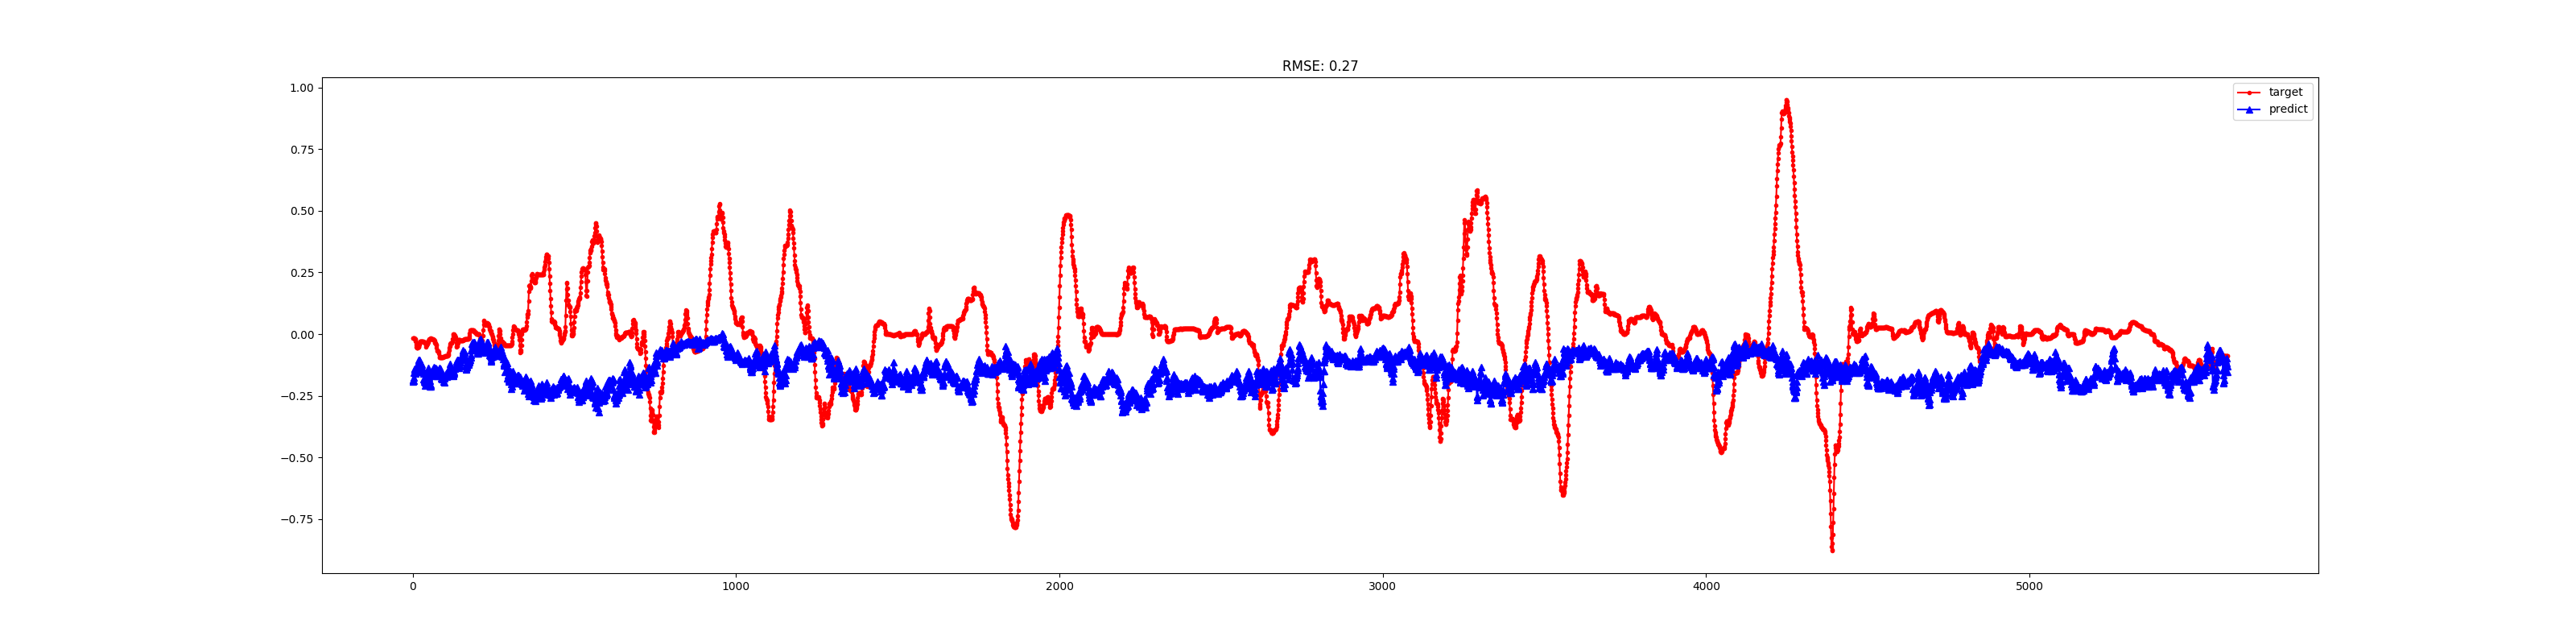
\includegraphics[width=1.5\textwidth, center]{rmse/1} 
    \caption{MUNIT}
\end{figure}
\begin{figure}[h]
    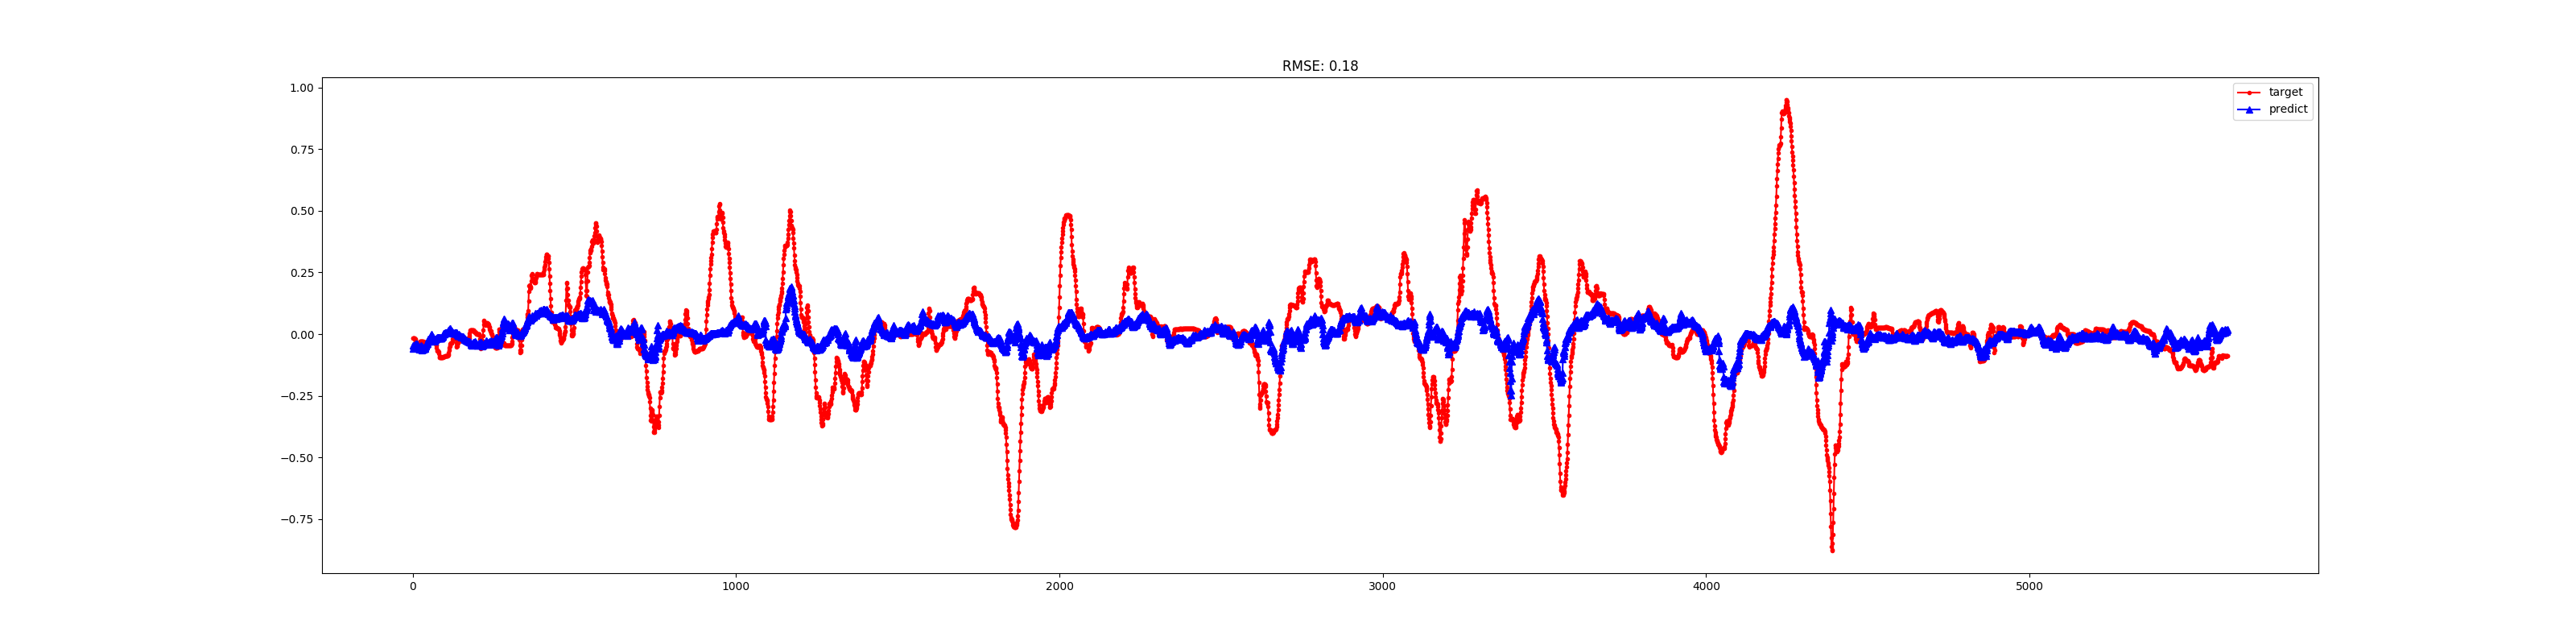
\includegraphics[width=1.5\textwidth, center]{rmse/2} 
    \caption{CycleGAN}
\end{figure}
\begin{figure}[h]
    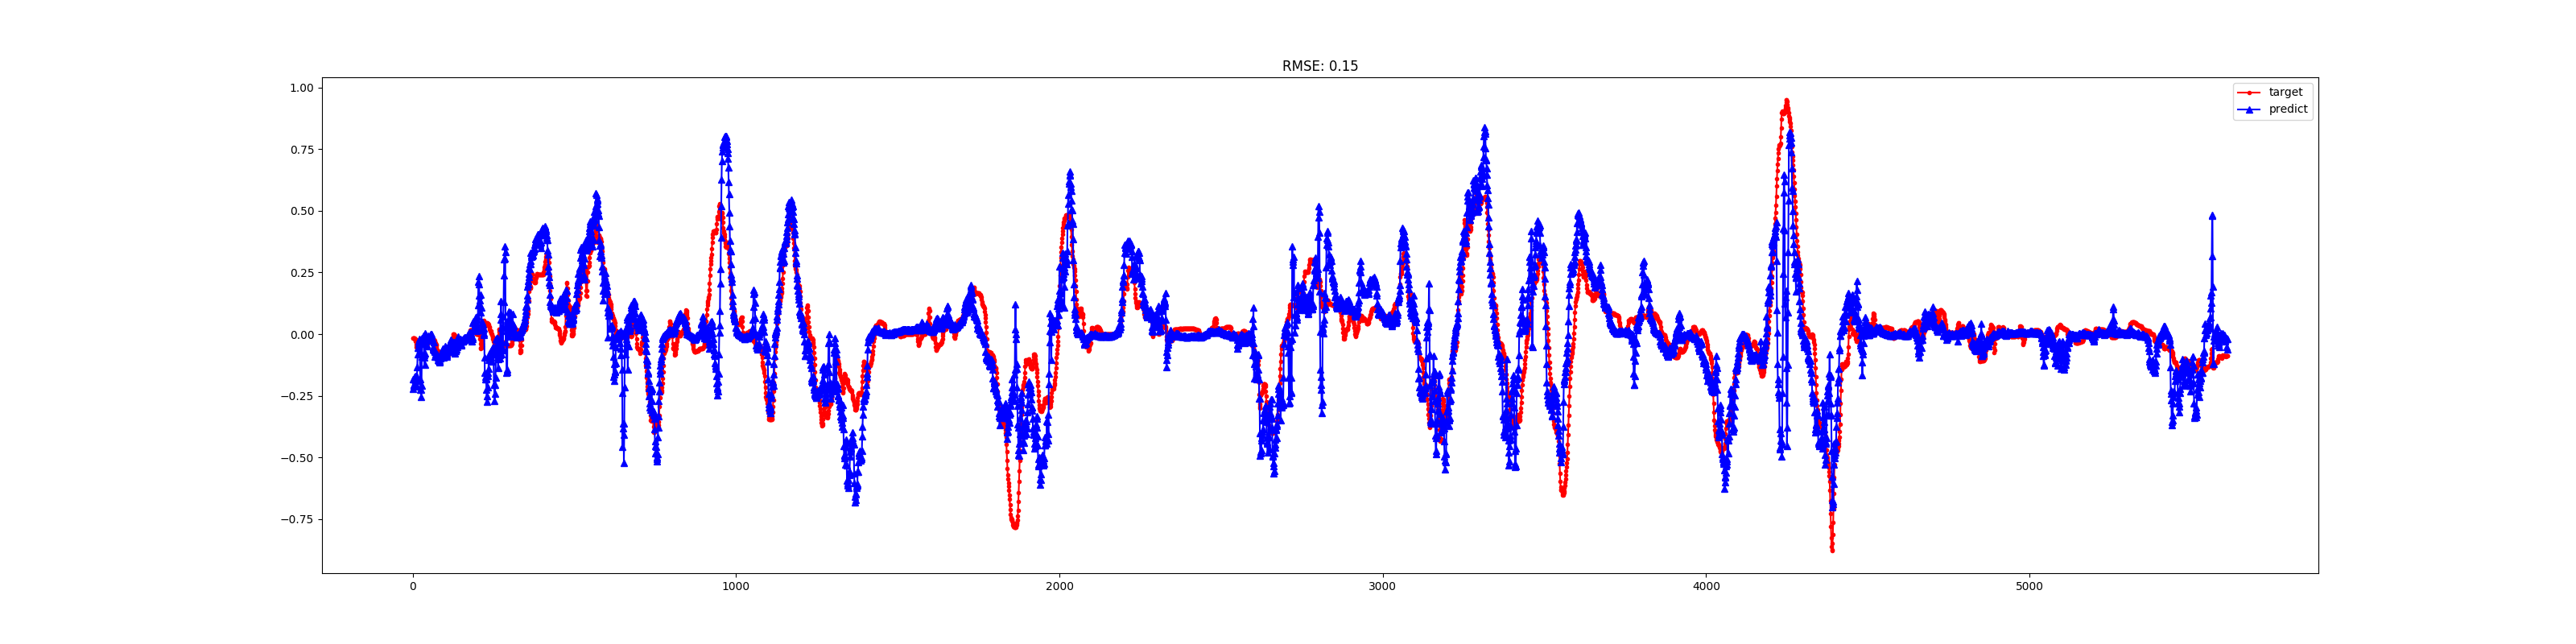
\includegraphics[width=1.5\textwidth, center]{rmse/3} 
    \caption{EBGAN}
\end{figure}
\begin{figure}[h]
    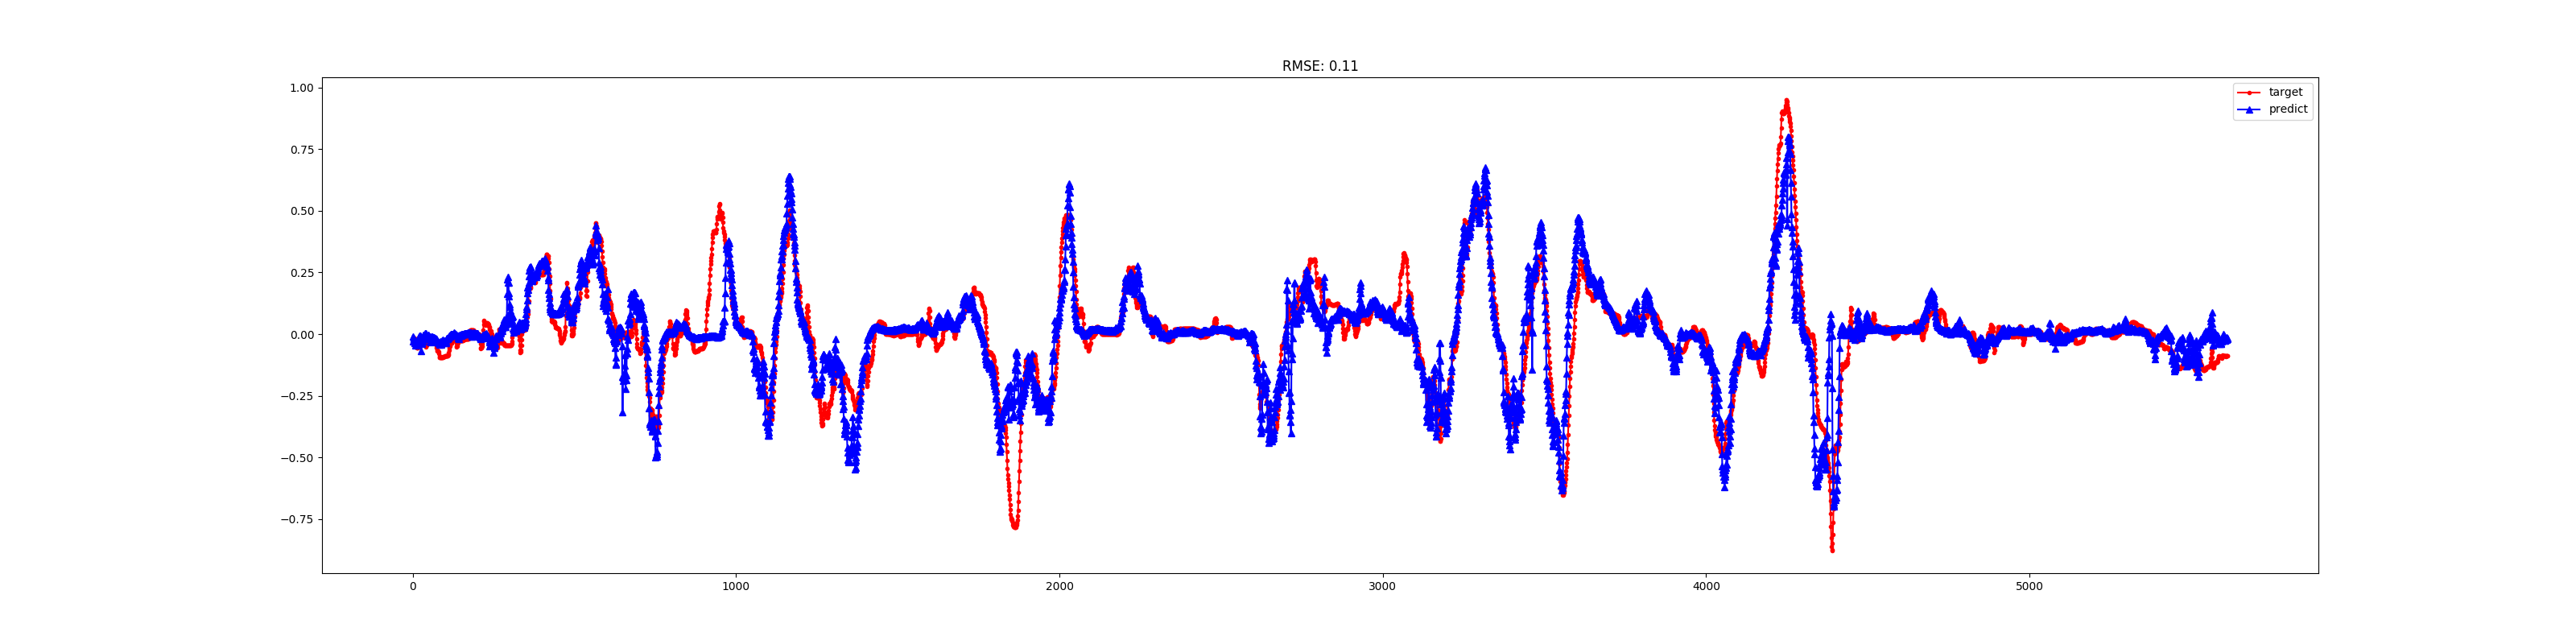
\includegraphics[width=1.5\textwidth, center]{rmse/4} 
    \caption{AdaIN Style}
\end{figure}
\begin{figure}[h]
    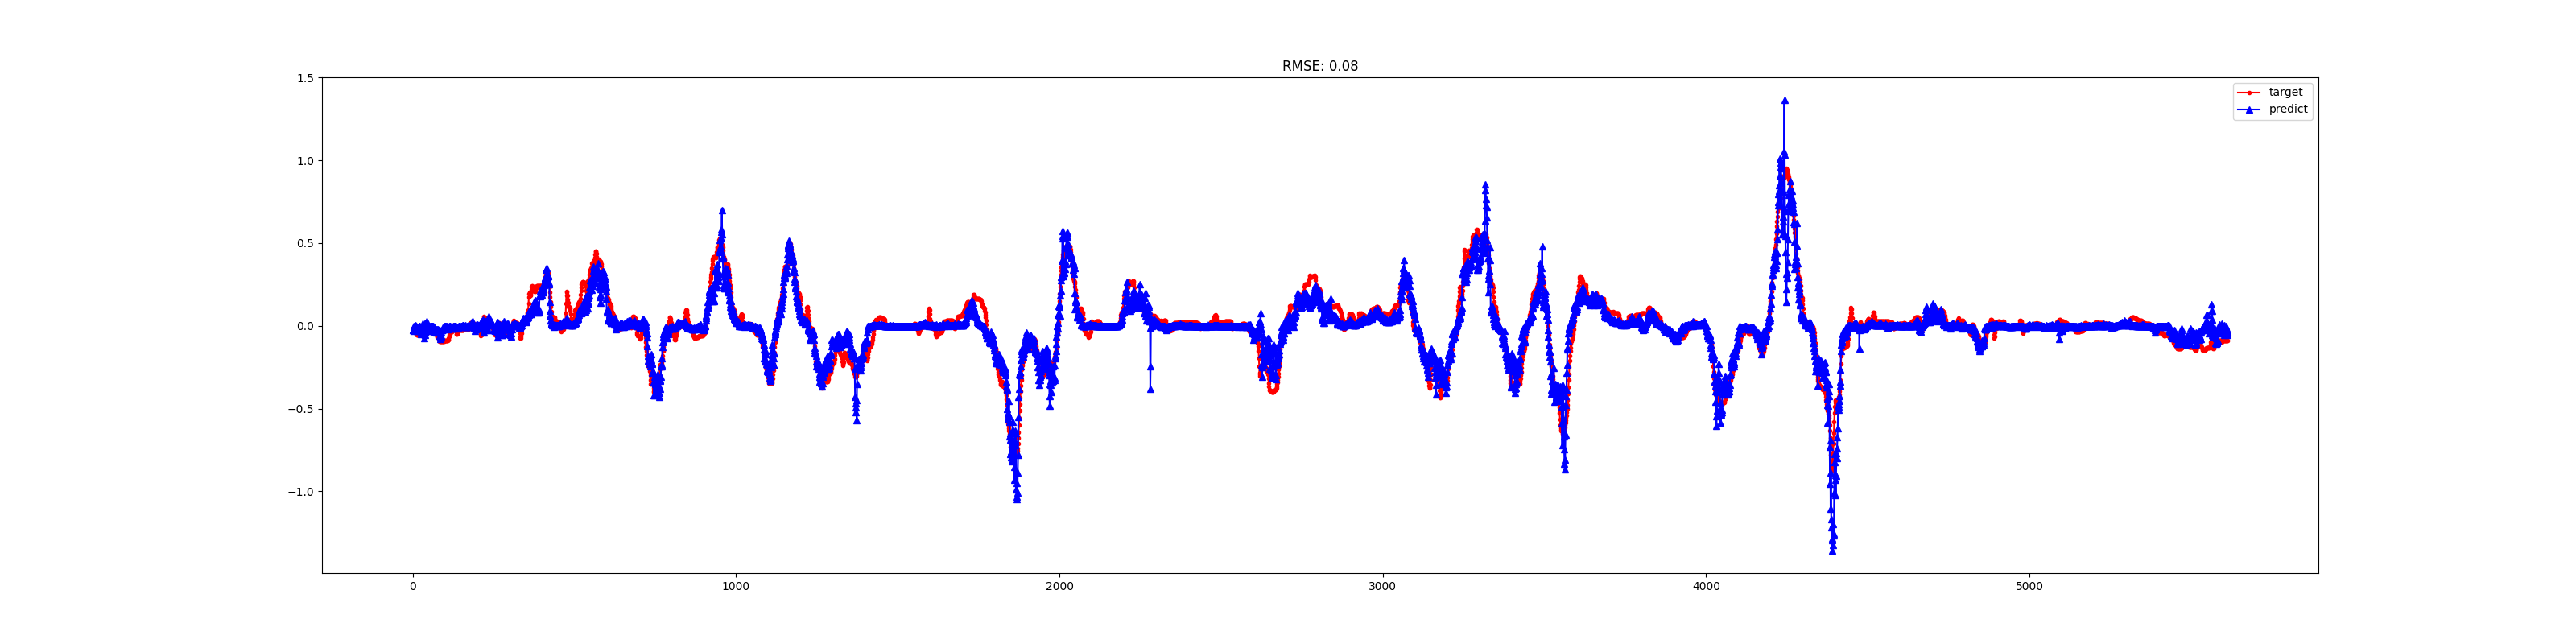
\includegraphics[width=1.5\textwidth, center]{rmse/5} 
    \caption{Deep Photo Style}
\end{figure}
\begin{figure}[h]
    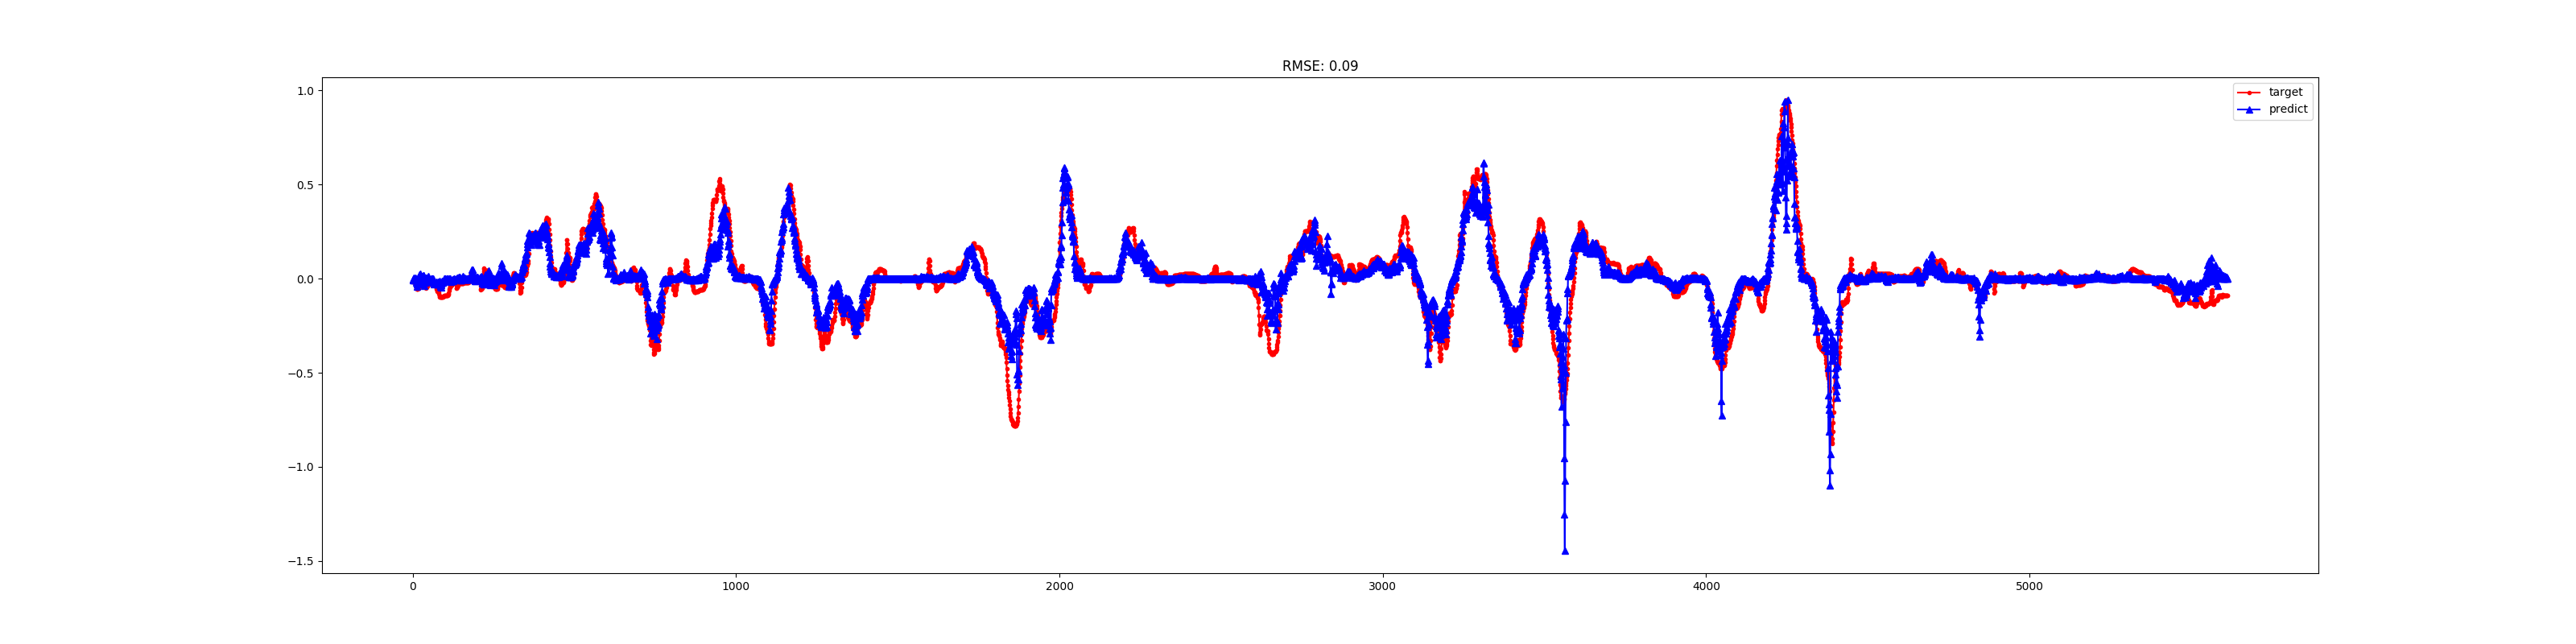
\includegraphics[width=1.5\textwidth, center]{rmse/6} 
    \caption{Fast Photo Style}
\end{figure}
\begin{figure}[h]
    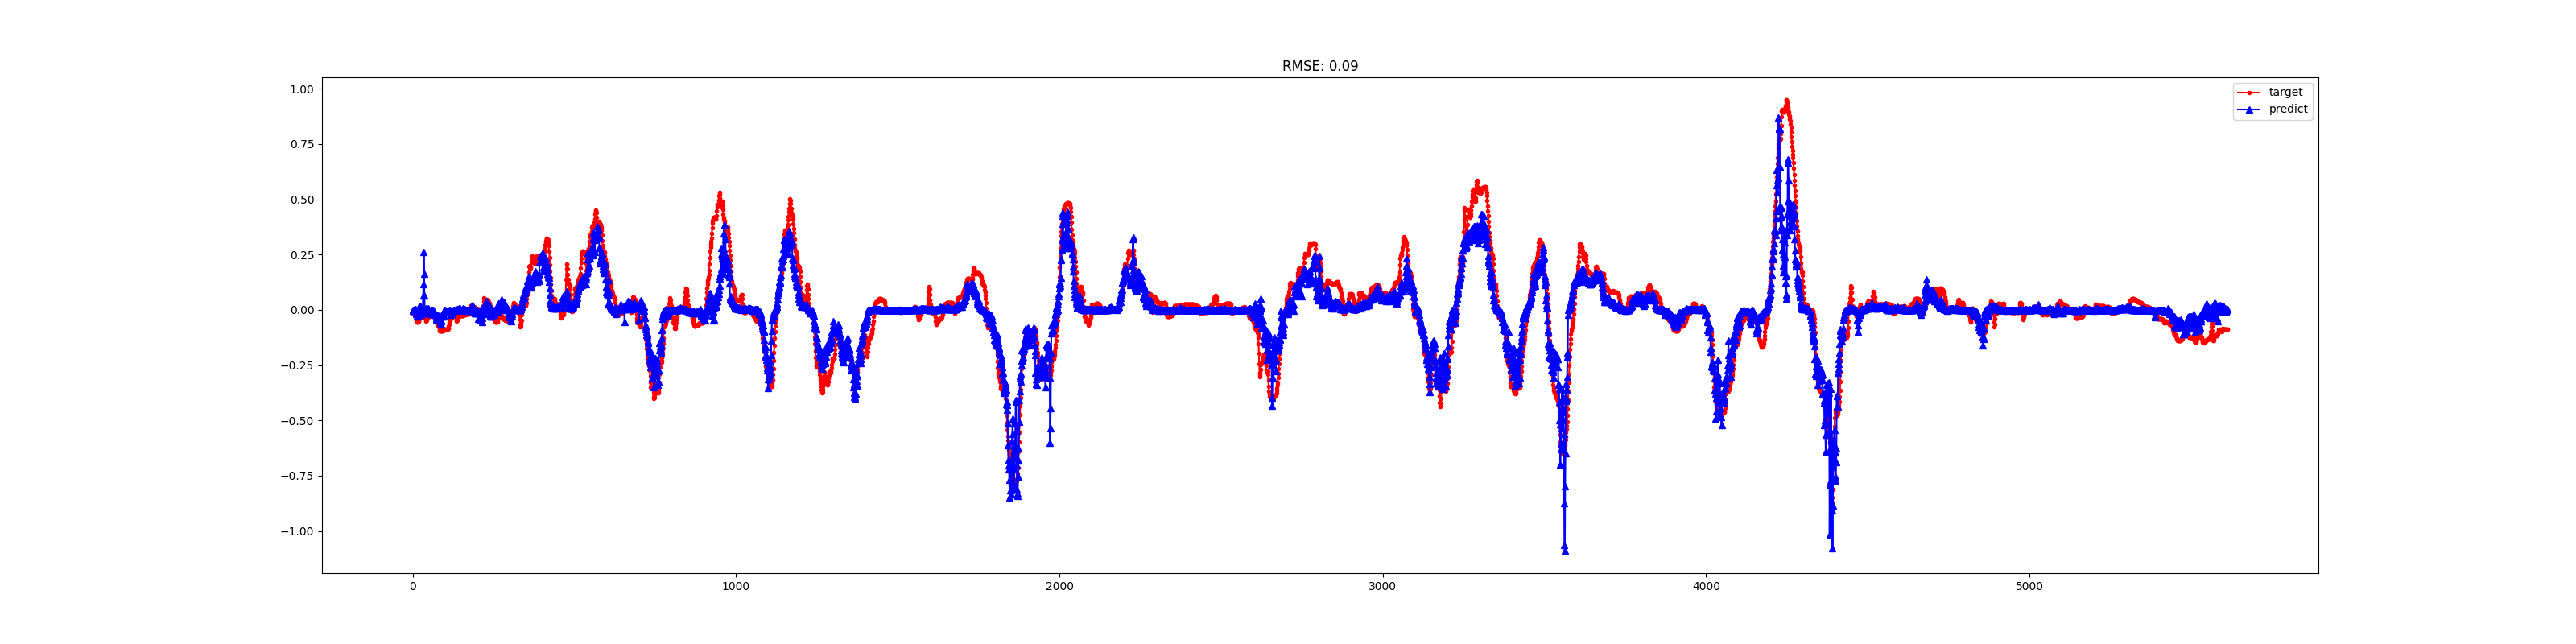
\includegraphics[width=1.5\textwidth, center]{rmse/7} 
    \caption{Fast Neural Transfer}
\end{figure}
\begin{figure}[h]
    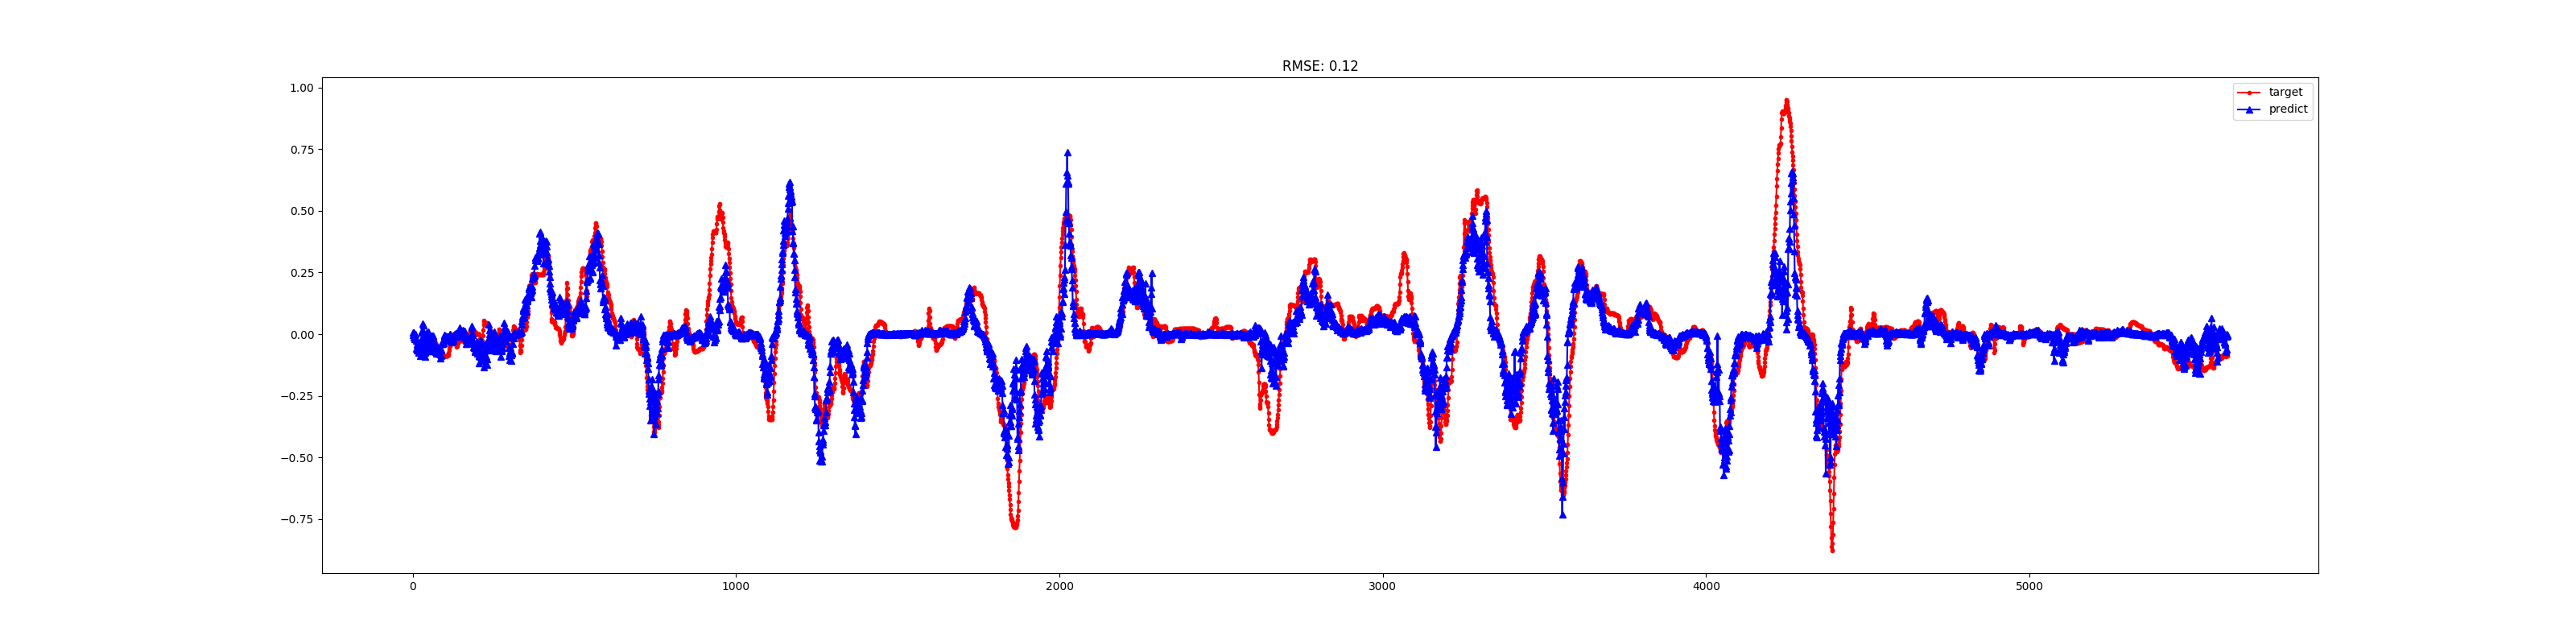
\includegraphics[width=1.5\textwidth, center]{rmse/8} 
    \caption{Texture Nets}
\end{figure}
\end{appendix}
\include{back/publications}    % 所发文章
\include{back/ceindex}    % 索引, 根据自己的情况添加或者不添加,选择自动添加或者手工添加。
\authorization %授权
%\authorization[saomiao.pdf] %添加扫描页的命令,与上互斥
% !Mode:: "TeX:UTF-8"
\begin{acknowledgements}
衷心感谢导师张煜群教授对本人的精心指导。他的言传身教将使我终生受益。

……

感谢哈工大\LaTeX\ 论文模板\hithesis\ !

\end{acknowledgements}
 %致谢
\include{back/resume}          % 博士学位论文有个人简介

%本科书序为:
%% !Mode:: "TeX:UTF-8" 
\begin{conclusions}

本文主要针对自动驾驶系统的测试用例,即路况图片的合成技术,围绕对抗生成网络和图像转换技术展开的实证研究。
经过对大量的深度学习模型实验与模型排除后,最后进行的实验数据统计的模型有8个:MUNIT,CycleGAN,EBGAN,AdaIN Style,Deep Photo Style,Fast Photo Style,Fast Neural Transfer,Texture Nets。

在实验的数据统计与总结中,我们提出了3个模型实验结果的比较指标:模型训练时间、FID值和方向盘拐角差。希望通过这3个指标综合、客观的评价比较出每个模型在路况图片转换中的性能优劣。在最终的实验数据以及我们选择的实验模型范围中来看,图像转换技术大类要由于对抗生成网络大类的模型。我们分析原因主要有有两点:

对抗生成网络的性能对训练数据集很敏感,且对数据集图片质量的要求很高,即需要内容数据集和样式数据集的图片内容结果十分接近。而满足要求的数据集往往需要专门的数据集采集工作,成本较高。而图像转换技术主要是对图像的像素色彩和明暗度做修改,所以对数据集的要求没有对抗生成网络的高,且在我们采集的结果数据中,各项指标数据都要优于对抗生成网络。

其次图像转换技术合成最终的图片中,会尽量保持原图片中的结构内容特征,所以对自动驾驶系统的行为干扰会比较小。

本研究的数据和成果基于文章中展开的研究对各个模型在图像转换性能上对提出的指标展开了定量的分析和比较,希望能对以后从事自动驾驶测试的技术人员,在图像转换技术模型选型上能够给出有价值的参考意见。

\end{conclusions}
   % 结论
%\bibliographystyle{hithesis}
%\bibliography{reference}
%\authorization %授权
%%\authorization[saomiao.pdf] %添加扫描页的命令,与上互斥
%% !Mode:: "TeX:UTF-8"
\begin{acknowledgements}
衷心感谢导师张煜群教授对本人的精心指导。他的言传身教将使我终生受益。

……

感谢哈工大\LaTeX\ 论文模板\hithesis\ !

\end{acknowledgements}
 %致谢
%\begin{appendix}%附录
%\input{body/appendix01}%本科生翻译论文
%\end{appendix}

\end{document}
